\section{Durchführung}
\label{sec:Durchführung}

In diesem Abschnitt werden der Versuchsaufbau und die Versuchsdurchführung beschrieben.

\subsection{Versuchsaufbau}

In \autoref{fig:aufbau} ist der Aufbau des Versuchs schematisch dargestellt.
\begin{figure}[H]
    \centering
    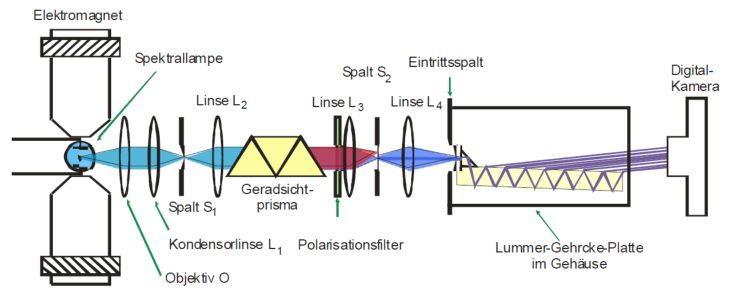
\includegraphics[width=\textwidth]{graphics/aufbau.JPG}
    \caption{Schematischer Aufbau der Messapparatur. \cite{v27}}
    \label{fig:aufbau}
\end{figure}

Wie zu sehen ist besteht der Versuchsaufbau aus der Cd-Lampe, die im Magnetfeld eines Elektromagneten positioniert ist sowie aus mehreren Linsen und Spalten, die der Fokussierung des Lichts dienen. Das Prisma spaltet das Licht in die unterschiedlichen Wellenlängen auf und der Polarisationsfilter wählt die Polarisationsrichtung aus. Die Lummer-Gehrcke-Platte am Ende des Versuchsaufbaus sorgt durch die konstruktive Interferenz der Lichtstrahlen an ihren planparallelen Platten für eine deutlich höhere Auflösung der Messung. Das so erzeugte Interferenzmuster wird schließlich mit einer Digitalkamera aufgenommen.

\subsection{Messprogramm}

Vor dem Beginn der Messungen muss das Magnetfeld geeicht werden. Dazu wird die Magnetfeldstärke in Abhängigkeit vom Feldstrom gemessen, sodass später nur noch die Stromstärke verändert werden muss. Die Messung der Magnetfeldstärke wird mit einer Hall-Sonde durchgeführt, welche möglichst mittig im Magnetfeld des Elektromagneten positioniert werden muss. \\
\newline
Im nächsten Schritt ist es wichtig den gesamten Messaufbau genau zu justieren. Dazu müssen die verschiedenen optischen Instrumente nacheinander so justiert werden, dass ein möglichst scharfes Bild auf das nächste Instrument fällt. Wennn die Justierung zu ungenau erfolgt, kann am Ende kein scharfes Bild mit der Digitalkamera aufgenommen werden. \\
\newline
Mit dem Spalt S2 kann eine der durch das Prisma separierten Wellenlängen ausgewählt werden und durch die Stellung des Polarisators wird anschließend einer der Übergänge ausgeblendet. Dann wird das Magnetfeld eingeschaltet, um die Aufspaltung der Spektrallinien beobachten zu können, welche schließlich mit der Digitalkamera aufgenommen wird. \\
Dieses Vorgehen wird einmal für die rote Linie und einmal für die blaue Linie der Cd-Lampe durchgeführt. Bei der blauen Linie ist zu beachten, dass die Aufspaltung sowohl für die $\pi$- als auch für die $\sigma$-Linie aufgenommen werden muss. Dabei ist es wichtig, dass die passenden Magnetfeldstärken für die unterschiedlichen Aufspaltungen genutzt werden. 